\scanpage{66}
\mspage{32}
$3^\circ)$ \uline{Cas \unsure{de|des}} $\widehat M^!_{0,5}$, ou $\widehat M_{0,I}$
\diagram{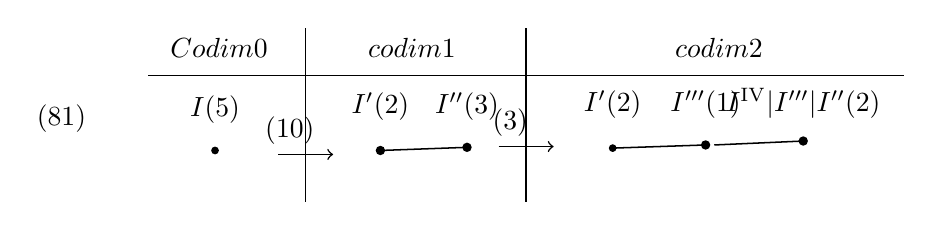
\begin{tikzpicture}[x=1cm,y=1cm,line width=.55pt]
\node at (-1.1,.4) {$(81)$};
\draw (0,.95)--(9.6,.95);
\draw (2,1.55)--(2,-.65);
\draw (4.8,1.55)--(4.8,-.65);
\node at (.9,1.3) {$\text{Codim }0$};
\node at (3.35,1.3) {$\text{codim }1$};
\node at (7.25,1.3) {$\text{codim }2$};
\fill (.85,0) circle (1.4pt);
\node[above] at (.85,.22) {$I(5)$};
\draw[->] (1.65,-.05)--(2.35,-.05);
\node[above] at (1.8,-.05) {$(10)$};
\draw (2.95,0)--(4.05,.04);
\fill (2.95,0) circle (1.7pt);
\fill (4.05,.04) circle (1.7pt);
\node[above] at (2.95,.26) {$I'(2)$};
\node[above] at (4.05,.26) {$I''(3)$};
\draw[->] (4.45,.05)--(5.15,.05);
\node[above] at (4.6,.05) {$(3)$};
\draw (5.9,.03)--(7.08,.07);
\draw (7.19,.07)--(8.32,.12);
\fill (5.9,.03) circle (1.4pt);
\fill (7.08,.07) circle (1.7pt);
\fill (8.32,.12) circle (1.7pt);
\node[above] at (5.9,.28) {$I'(2)$};
\node[above] at (7.08,.28) {$I'''(1)$};
\node[above] at (8.32,.28) {$\unsure{I^{\mathrm{IV}}|I'''|I''}(2)$};
\end{tikzpicture}}
Dans \unsure{de|le} $\widehat M^!_{0,5}$ il y a dix ``diviseurs à l'infini'', dont chacun est un $\widehat M^!_{0,4}$ \deleted{\unsure{$\simeq\mathbb P$}}, \deleted{\unsure{$\mathbb P^1_{0,3}\mathfrak S_3$}} \inserted{(plus précisément, un $\widehat M_{0,I''(3)\amalg(*)}\simeq(\mathbb P^1_{I''})_{\mathbb Z}$)} (ayant comme on avait vu, et \unsure{avait|aurait}) trois points à l'infini --- les pts à l'infini sont en nb total $\frac{30}{2}=15$, correspondant aux partitions de $I(5)$ de type $(2,2,1)$, alors que les diviseurs à l'infini correspondent aux parties \inserted{$I'$} de $I$ de cardinal $2$. Deux tels diviseurs, correspondant à des parties $I',I''\in\mathfrak P_2(I)$, se rencontrent sss \deleted{elles} on a $I'\cap I''=\phi$, i.e. \unsure{sss|\deleted{sss}} $I',I''$ et $I\smallsetminus(I'\cup I'')$ forment justement une partition de $I$ de type $(2,2,1)$.
\margin{$\mathbb P^1_{I''}\overset{\mathrm{def}}{=}\mathbb P^1_{\mathbb Z}\wedge_{\mathfrak S_3}\operatorname{Isom}(\{0,1,\infty\},I'')$}

D'après l'étude combinatoire de l'icosaèdre, \unsure{choisissant|choisissons} une orientation de $I$ --- ce qui détermine un icosaèdre orienté, ou encore un icos. gauche) les $10$ diviseurs à l'infini \deleted{\unsure{en ordre}} de $\widehat M_{0,I}$, i.e. les \inserted{$10$} \unsure{elmts|elts} de $\mathfrak P_2(I)$, \inserted{ou (par} \deleted{\unsure{correspon-}}
\margin{65}
